%=============================================================================%
% Author: 	John Joseph Valletta, Bram Kuijper
% Date: 	14/03/2017, 04/03/2019
% Title: 	Python workshop: functions, modules
%=============================================================================%

%=============================================================================%
% Preamble
%=============================================================================%
% Libraries

\documentclass[xcolor=table]{beamer}
\usepackage{beamerthemeshadow}
\usepackage{helvet}
\usepackage[]{graphicx}
\usepackage{array}
\usepackage{color}
\definecolor{dkgreen}{rgb}{0,0.6,0}
\definecolor{gray}{rgb}{0.5,0.5,0.5}
\definecolor{mauve}{rgb}{0.58,0,0.82}
\definecolor{deepblue}{rgb}{0,0,0.5}
\definecolor{deepred}{rgb}{0.6,0,0}
\definecolor{deepgreen}{rgb}{0,0.5,0}
\definecolor{lightgray}{rgb}{0.92,0.92,0.92}
\usepackage{listings} % to insert code
\usepackage{textpos} % textblock
\usepackage{dirtree} % textblock
\usepackage{hyperref}
\hypersetup{colorlinks=true, urlcolor=blue, linkcolor=black} 
% Listing set up
% bash
\lstdefinestyle{bash}{
language=bash,                     % the language of the code
basicstyle=\scriptsize\ttfamily,       % the size of the fonts that are used for the code
numbers=none,%left,                   % where to put the line-numbers
numberstyle=\tiny\color{gray},  % the style that is used for the line-numbers
stepnumber=1,                   % the step between two line-numbers. If it's 1, each line
                          % will be numbered
numbersep=5pt,                  % how far the line-numbers are from the code
backgroundcolor=\color{lightgray},  % choose the background color. You must add \usepackage{color}
showspaces=false,               % show spaces adding particular underscores
showstringspaces=false,         % underline spaces within strings
showtabs=false,                 % show tabs within strings adding particular underscores
frame=lines,%single,                   % adds a frame around the code
rulecolor=\color{black},        % if not set, the frame-color may be changed on line-breaks within not-black text (e.g. commens (green here))
tabsize=2,                      % sets default tabsize to 2 spaces
captionpos=b,                   % sets the caption-position to bottom
breaklines=true,                % sets automatic line breaking
breakatwhitespace=false,        % sets if automatic breaks should only happen at whitespace
title=\lstname,                 % show the filename of files included with \lstinputlisting;
                          % also try caption instead of title
keywordstyle=\color{blue},      % keyword style
commentstyle=\color{dkgreen},   % comment style
stringstyle=\color{mauve},      % string literal style
escapeinside={\%*}{*)},         % if you want to add a comment within your code
morekeywords={}            % if you want to add more keywords to the set
}

% Python
\lstdefinestyle{python}{
language=python,
formfeed=\newpage,
basicstyle=\scriptsize\ttfamily,
commentstyle=\color{deepgreen},%\color{gray},
numbers=left,
numberstyle=\tiny\color{gray},
stepnumber=1,
numbersep=5pt,
backgroundcolor=\color{lightgray},%\color{white},
showspaces=false,
showstringspaces=false,
showtabs=false,
frame=lines,
tabsize=4,
captionpos=b,
breaklines=true,
breakatwhitespace=false,
title=\lstname,
escapeinside=||,
keywordstyle=\color{deepblue},
emphstyle=\color{deepred},
stringstyle=\color{deepgreen}
%morekeywords={models, lambda, forms}
}

\graphicspath{ {../img/} }
\title[Python for scientific research]{Python for scientific research}
\subtitle{Functions and modules}
\author{Bram Kuijper}
\institute[]{University of Exeter, Penryn Campus, UK}
\titlegraphic{
\hfill

\includegraphics[width=\textwidth, keepaspectratio]{logo.jpg}}
%=============================================================================%
%=============================================================================%
% Start of Document
%=============================================================================%
%=============================================================================%
\begin{document}

%=============================================================================%
%=============================================================================%
\begin{frame}
\titlepage
\end{frame}

%=============================================================================%
%=============================================================================%
\begin{frame}{What we've done so far}

	\begin{enumerate}\addtolength{\itemsep}{1\baselineskip}
		\item Declare variables using built-in data types and execute operations
		on them
		\item Use flow control commands to dictate the order in which commands are run
		and when
		\item \textbf{Next}: Encapsulate programs into reusable functions, modules and packages
	\end{enumerate}

\end{frame}

%=============================================================================%
%=============================================================================%
\begin{frame}[fragile]
\frametitle{Motivation}

\begin{itemize}\addtolength{\itemsep}{-1\baselineskip}
	\item<1-> Imagine we wrote a series of commands to perform a particular task, for example,
	searching for a motif within a DNA sequence string 

\begin{lstlisting}[style=python]
motif = "ggatcc" # sequence to search for
DNA = "acgtgtaaccaaggatccacccgttttaaacctgtgtgggatcc" # my DNA
index = 0 # index of where to start looking for motif
indices = [] # result; list of indices where motif is
while index != -1: # -1 implies no match
    index = DNA.find(motif, index)
    if index != -1:
        indices.append(index)
        index += 1
\end{lstlisting}

	\item <2-> We are now presented with a new DNA sequence and/or a different motif, what do we do? 
	\begin{enumerate}\addtolength{\itemsep}{0.5\baselineskip}
		\item<2-> Copy and paste the above program and change \texttt{motif} and \texttt{DNA}
		\item<3-> \textbf{Encapsulate the commands into a reusable function}
	\end{enumerate}

\end{itemize}

\end{frame}

%=============================================================================%
%=============================================================================%
\begin{frame}{Anatomy of functions}

\begin{itemize}\addtolength{\itemsep}{0.5\baselineskip}
	\item<1-> Functions are ubiquitous in programming, enabling us to invoke the same
	function over and over again; \textbf{reusability}

	\item<2-> Using functions allow us to ``hide" complexity (abstraction), 
	making it easier to build complex programs, as we only need to 
	worry about how to \textbf{use} the function rather than how it \textbf{works}
	on the inside

	\item<3-> In a nutshell, functions take a number of \textbf{input} arguments
	(e.g \texttt{DNA, motif}) and return an \textbf{output} (e.g \texttt{indices})
\end{itemize}
\vfill
\begin{center}
	\visible<3->{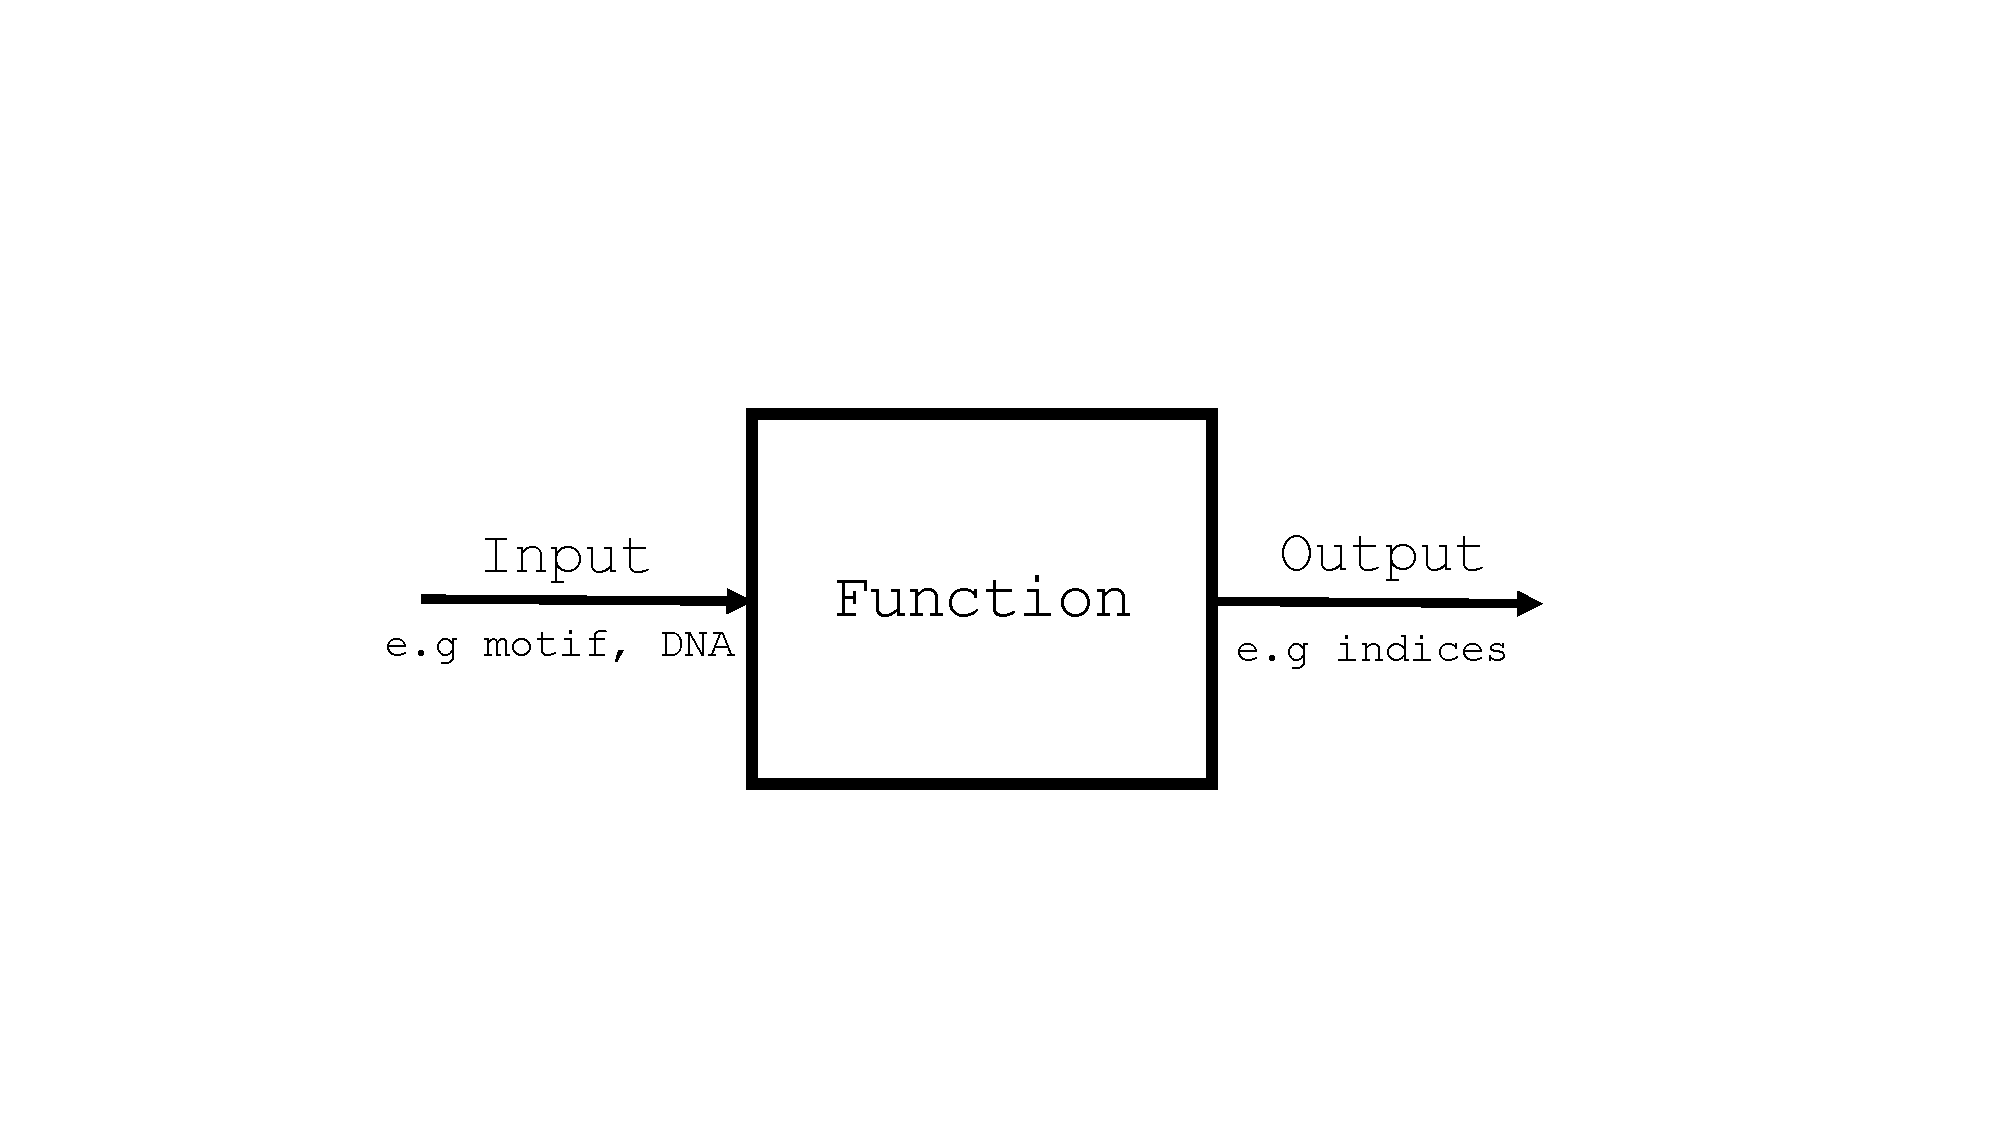
\includegraphics[width=0.7\textwidth]{function.pdf}}
\end{center}

\end{frame}

%=============================================================================%
%=============================================================================%
\begin{frame}[fragile]
\frametitle{Simple functions}

\begin{itemize}[leftmargin=*]
\item<1->Sum two numbers
\begin{lstlisting}[style=python]
def mysum(x, y):
    return x + y

# Call function
out = mysum(10, 2) # out = 12
\end{lstlisting}

\item<2->Sum and divide two numbers
\begin{lstlisting}[style=python]
def sum_and_divide(x, y):
    return x+y, x/y

# Call function
out1, out2 = sum_and_divide(10, 2) # out1 = 12, out2 = 5
\end{lstlisting}

\end{itemize}
\end{frame}

%=============================================================================%
%=============================================================================%
\begin{frame}[fragile]
\frametitle{Simple functions}

\begin{itemize}[leftmargin=*]
\item<1->Sum, and divide two numbers after checking for division by zero
\begin{lstlisting}[style=python]
def sum_and_divide(x, y):
    # Compute sum
    mySum = x + y
    
    # Compute division only if y is not zero
    if y != 0:
        myDiv = x/y
    else:
        myDiv = None
        
    # Return sum and division results
    return mySum, myDiv

# Call function
out1, out2 = sum_and_divide(10, 0) # out1 = 10, out2 = None
\end{lstlisting}
\end{itemize}

\end{frame}

%=============================================================================%
%=============================================================================%
\begin{frame}{Note}

\begin{itemize}\addtolength{\itemsep}{1.5\baselineskip}

\item<1-> Python functions lack \{ \} used in many other languages (e.g R, C); \textbf{indentation} is everything!

\item<2-> It is good practice to \texttt{return} something after a function call; if you don't
Python will return an object of type \texttt{None}

\item<3-> Terminology
\begin{enumerate}\addtolength{\itemsep}{.5\baselineskip}
	\item \textbf{Parameters}: the variable names defined in the function definition
	\item \textbf{Arguments}: the values supplied to a function when it is called 
\end{enumerate}
\end{itemize}

\end{frame}

%=============================================================================%
%=============================================================================%
\begin{frame}[fragile]
\frametitle{Finding a motif within a DNA sequence}

\begin{lstlisting}[style=python]
motif = "ggatcc" # sequence to search for
DNA = "acgtgtaaccaaggatccacccgttttaaacctgtgtgggatcc" # my DNA
index = 0 # index of where to start looking for motif
indices = [] # result; list of indices where motif is
while index != -1: # -1 implies no match
    index = DNA.find(motif, index)
    if index != -1:
        indices.append(index)
        index += 1
\end{lstlisting}

\end{frame}

%=============================================================================%
%=============================================================================%
\begin{frame}[fragile]
\frametitle{Wrap code into a function}

\begin{lstlisting}[style=python]
def find_motif(DNA, motif):
    index = 0 # index of where to start looking for motif
    indices = [] # result; list of indices where motif is
    while index != -1: # -1 implies no match
        index = DNA.find(motif, index)
        if index != -1:
            indices.append(index)
            index += 1
    return indices # return an output; indices
\end{lstlisting}

\end{frame}

%=============================================================================%
%=============================================================================%
\begin{frame}[fragile]
\frametitle{Using default argument values}

\begin{lstlisting}[style=python]
def find_motif(DNA, motif="gaatca"):
    index = 0 # index of where to start looking for motif
    indices = [] # result; list of indices where motif is
    while index != -1: # -1 implies no match
        index = DNA.find(motif, index)
        if index != -1:
            indices.append(index)
            index += 1
    return indices # return an output; indices
\end{lstlisting}

\end{frame}

%=============================================================================%
%=============================================================================%
\begin{frame}[fragile]
\frametitle{Always include a documentation string}

\begin{lstlisting}[style=python]
def find_motif(DNA, motif="gaatca"):
    """
    Finds a motif within a DNA sequence and returns a list 
    of start indices
    
    Parameters
    ----------
    motif : a string to be matched 
    DNA : a string containing the DNA sequence to be searched
    
    Returns
    -------
    indices : list of start indices where motif is located
    """
    index = 0 # index of where to start looking for motif
    indices = [] # result; list of indices where motif is
    while index != -1: # -1 implies no match
        index = DNA.find(motif, index)
        if index != -1:
            indices.append(index)
            index += 1
    return indices # return an output; indices
\end{lstlisting}

\end{frame}

%=============================================================================%
%=============================================================================%
\begin{frame}[fragile]
\frametitle{Calling functions}


\begin{enumerate}\addtolength{\itemsep}{-0.4\baselineskip}
\begin{lstlisting}[style=python]
# Example
motif1 = "ggatcc" # sequence to search for
motif2 = "aacctg" # another sequence to search for
DNA = "acgtgtaaccaaggatccacccgttttaaacctgtgtgggatcc"
\end{lstlisting}
\vspace{-0.5cm}
\item<1-> By argument order/position
\begin{lstlisting}[style=python]
indices1 = find_motif(DNA, motif1)
\end{lstlisting}

\item<2-> By argument keyword (preferred)
\begin{lstlisting}[style=python]
indices2 = find_motif(motif=motif2, DNA=DNA)
\end{lstlisting}

\item<3-> Using default arguments
\begin{lstlisting}[style=python]
indicesDefault = find_motif(DNA)
\end{lstlisting}

\end{enumerate}

\end{frame}

%=============================================================================%
%=============================================================================%
\begin{frame}[fragile]
\frametitle{Modules}

\begin{itemize}
	\item We will typically write functions to perform a variety of related
	tasks

\begin{lstlisting}[style=python]
def complement(DNA):
    """
    Return the complement of a DNA sequence 
    """
    <Your funky code>
    return output

def reverse_complement(DNA):
    """
    Return the reverse complement of a DNA sequence 
    """
    <Your funky code>
    return output 

def find_motif(motif, DNA):
    """
    Finds a motif within a DNA sequence 
    """
    <Your funky code>
    return output 
...
\end{lstlisting}

\end{itemize}
\end{frame}

%=============================================================================%
%=============================================================================%
\begin{frame}[fragile]
\frametitle{Modules}

\begin{itemize}\addtolength{\itemsep}{1.2\baselineskip}
	
	\item<1-> \textbf{Modules} let us reuse functions in any program 
	without the need to redefine them (read: copy and paste)

	\item<2-> Grouping functions by topic makes our code easier to use, understand and debug

	\item<3-> \textbf{Modules} are simply Python files (\texttt{.py}) that contain
	definitions of functions and variables related to some specific theme

	\item<4-> For example let us save the previously defined DNA sequence functions
	to a file called \texttt{dna\_utils.py}; our new \textbf{module}
	 

\end{itemize}
\end{frame}

%=============================================================================%
%=============================================================================%
\begin{frame}[fragile]
\frametitle{Importing modules}

\begin{itemize}\addtolength{\itemsep}{\baselineskip}

	\item We can access functions from modules by using the \texttt{import} command
	and '.' notation

\begin{lstlisting}[style=python]
# Preamble
import dna_utils

# Declare some variables
motif = "aacctg" # sequence to search for
DNA = "acgtgtaaccaaggatccacccgttttaaacctgtgtgggatcc" # my DNA

# Return complement of DNA sequence
compDNA = dna_utils.complement(DNA)

# Return reverse complement of DNA sequence
revCompDNA = dna_utils.reverse_complement(DNA)

# Find motif within DNA sequence 
indices = dna_utils.find_motif(DNA, motif)
\end{lstlisting}

\end{itemize}

\end{frame}

%=============================================================================%
%=============================================================================%
\begin{frame}{Packages}

\begin{itemize}\addtolength{\itemsep}{\baselineskip}
	\item<1-> What if I wrote the following modules?
	\begin{enumerate}
		\item<2-> \texttt{dna\_utils.py}: {\scriptsize functions for DNA sequences}
		\item<3-> \texttt{rna\_utils.py}: {\scriptsize functions for mRNA sequences}
		\item<4-> \texttt{protein\_utils.py}: {\scriptsize functions for protein coding sequences}
		\item<5-> \texttt{fasta\_utils.py}: {\scriptsize functions for FASTA files}
		\item<6-> \texttt{fastq\_utils.py}: {\scriptsize functions for FASTQ files}
		\item<6-> ...
	\end{enumerate}

	\item<7-> A \textbf{package} is a group of related modules that help us organise our code
	even further

	\item<8-> A \textbf{package} is a normal folder containing the Python file \texttt{\_\_init\_\_.py} 
	which tells Python that the folder contains modules  
\end{itemize}

\end{frame}

%=============================================================================%
%=============================================================================%
\begin{frame}{Hierarchical organisation: divide and conquer}

\begin{center}
	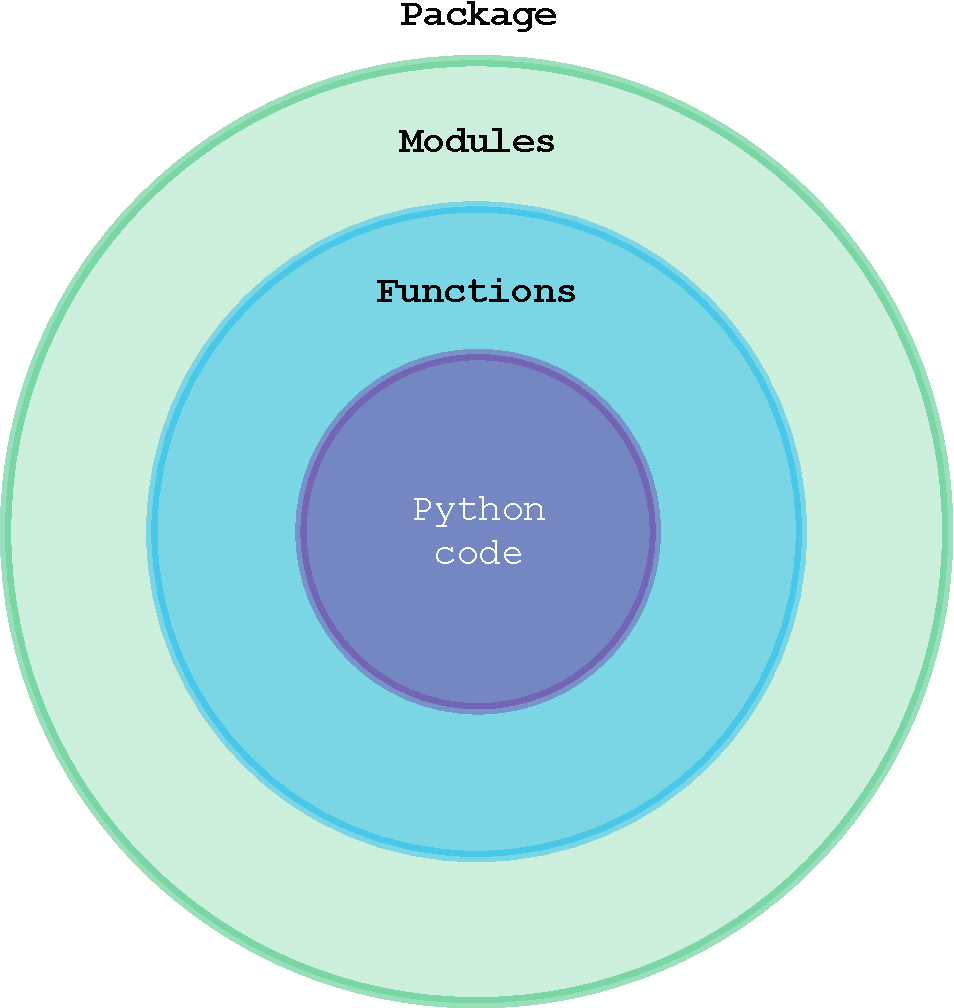
\includegraphics[width=0.62\textwidth, keepaspectratio]{package.pdf}
\end{center}

\end{frame}

%=============================================================================%
%=============================================================================%
\begin{frame}[fragile]
\frametitle{Package example}

\begin{itemize}
	\item This is what our genomics package could look like
\end{itemize}

\begin{columns}
\column{0.4\textwidth}

\dirtree{%
.1 genomics/.
.2 \_\_init\_\_.py.
.2 dna\_utils.py.
.2 rna\_utils.py.
.2 protein\_utils.py.
.2 fasta\_utils.py.
.2 fastq\_utils.py.
.2 ....
}

\column{0.6\textwidth}
\begin{lstlisting}[style=python]
import genomics.dna_utils

import genomics.rna_utils

import genomics.fasta_utils

...
\end{lstlisting}
\end{columns}

\end{frame}

%=============================================================================%
%=============================================================================%
\begin{frame}[fragile]
\frametitle{Package example}

\begin{itemize}
	\item Or we can organise it even further
\end{itemize}


\begin{columns}
\column{0.44\textwidth}

\dirtree{%
.1 genomics/.
.2 \_\_init\_\_.py.
.2 dna\_utils.py.
.2 rna\_utils.py.
.2 protein\_utils.py.
%
.2 fasta/.
.3 \_\_init\_\_.py.
.3 quality\_control.py.
.3 read\_write.py.
.3 ....
%
.2 fastq/.
.3 \_\_init\_\_.py.
.3 quality\_control.py.
.3 read\_write.py.
.3 ....
}

\column{0.56\textwidth}
\begin{lstlisting}[style=python]
import genomics.dna_utils

import genomics.rna_utils

import genomics.fasta.quality_control

import genomics.fasta.read_write

...
\end{lstlisting}
\end{columns}

\end{frame}

%=============================================================================%
%=============================================================================%
\begin{frame}[fragile]
\frametitle{Importing from a package}

\begin{itemize}

\item<1-> We can access functions from modules in a package by using the  
\texttt{from ... import ...} command and '.' notation
\begin{lstlisting}[style=python]
# Preamble
from genomics import dna_utils

# Return complement of DNA sequence
compDNA = dna_utils.complement(DNA)
\end{lstlisting}

\item<2-> Going one level down the hierarchy
\begin{lstlisting}[style=python]
# Preamble
from genomics.fastq import quality_control

# Check if "sample1.fastq" is a valid FASTQ file
flag = quality_control.validate("sample1.fastq")
\end{lstlisting}

\end{itemize}

\end{frame}

%=============================================================================%
%=============================================================================%
\begin{frame}[fragile]
\frametitle{Importing from a package}

\begin{itemize}

\item<1-> We can also import only the functions we need
\begin{lstlisting}[style=python]
# Preamble
from genomics.dna_utils import complement, reverse_complement

# Example
compDNA = complement(DNA) # complement
revCompDNA = reverse_complement(DNA) # reverse complement
\end{lstlisting}

\item<2-> Or rename the module/package upon importing
\begin{lstlisting}[style=python]
# Preamble
from genomics import dna_utils as util

# Example
compDNA = util.complement(DNA) # complement
revCompDNA = util.reverse_complement(DNA) # reverse complement
\end{lstlisting}

\end{itemize}

\end{frame}

%=============================================================================%
%=============================================================================%
\begin{frame}[fragile]
\frametitle{Warning}

\begin{itemize}\addtolength{\itemsep}{0.8\baselineskip}

\item <1-> We can import \textbf{all} functions and variables from a module as follows
\begin{lstlisting}[style=python]
# Preamble
from genomics.dna_utils import *

# Example
compDNA = complement(DNA) # complement
\end{lstlisting}
\vspace{-0.7cm}
\item<2-> \textbf{AVOID} using \texttt{import *}

\item<3-> ``\textbf{Explicit is better than implicit}" - {\scriptsize \textit{The Zen of Python}}

\item<4-> If you \texttt{import *} from several packages/modules you will get conflicts
if functions have the same name 

\item<5-> ``\textbf{Namespaces are one honking great idea}" - {\scriptsize \textit{The Zen of Python}}

\end{itemize}

\end{frame}

%=============================================================================%
%=============================================================================%
\begin{frame}{Final note}

\visible<1->{\begin{block}{MATLAB\textsuperscript\textregistered}
\begin{itemize}\addtolength{\itemsep}{0.2\baselineskip}
	\item Python packages are equivalent to MATLAB toolboxes
	\item Toolboxes are loaded to the global namespace/workspace
	\item There's an equivalent \texttt{import} function introduced recently
\end{itemize}
\end{block}}
\vfill
\visible<2->{\begin{block}{R}
\begin{itemize}\addtolength{\itemsep}{0.2\baselineskip}
	\item Python packages are equivalent to R libraries/packages 
	\newline
	e.g \texttt{library(tidyr)}
	\item Packages are loaded to the global namespace/workspace
	\item Using the double colon operator (\texttt{::}) conflicts can be avoided
	\newline
	e.g \texttt{tidyr::gather(...)}
\end{itemize}
\end{block}}

\end{frame}

%=============================================================================%
%=============================================================================%
% End of Document
%=============================================================================%
%=============================================================================%
\end{document}
